%% Used Compiler: pdfLaTeX / XeLaTeX
%% Diese Arbeit wurde unter Berücksichtigung der Hinweise_Abschlussarbeiten_22.11.2013.pdf, die durch das
%% Institut für Finanzwirtschaft an der TU-Braunschweig bereitgestellt wird, erstellt.

%-------------------------------------------
%% Zusätzliche Pakete werden geladen
%\documentclass[a4paper,12pt,titlepage]{article}  
\documentclass[a4paper, 12pt, titlepage]{scrartcl} % Schrift- und Papiergröße werden eingestellt  
\usepackage[top=3cm, bottom=3cm, left=2.5cm, right=2.5cm]{geometry} % Korrekturrand wird eingestellt
\usepackage[ngerman]{babel}             % Dokumentsprache wird auf deutsch gesetzt
\usepackage[onehalfspacing]{setspace}   % Zeilenabstand wird auf 1,5 gesetzt
\usepackage{color}                      % Ermöglicht die Änderung der Schriftfarbe
\usepackage{graphicx}                   % Ermöglicht das Einbinden von Bildern
\usepackage{fancyhdr}                   % Ermöglicht die freie Bearbeitung der Fuß und Kopfzeilen
\usepackage{tocloft}                    % Ermöglicht das anpassen des Inhaltsverzeichnisses
\usepackage{wrapfig}                    % Ermöglicht textumschlossene Abbildungen
\usepackage{array}                      % Ermöglicht das Anpassen von Tabellen

%-------------------------------------------
%% Fonteinstellungen abhängig vom Compiler
%% Quellen: https://en.wikibooks.org/wiki/LaTeX/Fonts
%%          https://www.sharelatex.com/learn/XeLaTeX
%%          https://tex.stackexchange.com/questions/12565/load-fonts-that-are-in-a-fonts-directory
\usepackage{ifxetex}                    % Ermöglicht das Prüfen ob XeLaTeX benutz wird
    \ifxetex
    \usepackage{fontspec}
    \defaultfontfeatures{Ligatures=TeX} % To support LaTeX quoting style
    \setmainfont[%                      % Times New Roman (aus Windows) wird als Standardschrift gesetzt
        Path = Fonts/,%                 % Dateien Pfad wird auf Fonts/ gesetzt
        BoldFont=timesbd.ttf,%
        ItalicFont=timesi.ttf,%
        BoldItalicFont=timesbi.ttf,%
        ]{times.ttf}
\else
    \usepackage[T1]{fontenc}            % Liefert die meisten Text-Zeichen für westeuropäische Sprachen
    \usepackage[utf8]{inputenc}         % Ermöglicht die direkte Eingabe der Umlaute
    \usepackage{mathptmx}               % Times wird als Standardschrift gesetzt
\fi

%-------------------------------------------
%% Pakete für das Erstellen von Refferenzen
\usepackage{varioref}
\usepackage{hyperref} % Erweitert die Referenzmöglichkeiten
\usepackage{cleveref}

%-------------------------------------------
%% Pakete für das Erstellen des Literaturverzeichnisses
\usepackage[babel,german=quotes]{csquotes}  % Verwendet die deutsche Art der Anführungszeichen
\usepackage[backend=biber, style=authoryear, citestyle=authoryear, maxitems=1]{biblatex}

\DefineBibliographyStrings{german}{%    % Verändert beim zitieren "u.a." zu "et al." und "und" zu "and"
  andothers = {et al.},
  and       = {and}
}
\addbibresource{10_literatur.bib}       % Fügt die Literaturverzeichnisdatei ein
\setlength{\bibitemsep}{10pt}           % Stellt den Zeilenabstand zwischen den Literaturverzeichnis Einträgen ein
%-------------
%% Erstellt ein Makro welches prüft ob die eingegebene Variable leer ist
\def\ifempty#1{% 
\def\temp{#1}%
\ifx\temp\empty%
}
%-------------
%% Erstellt mit \fcite ein Zitat in der Fußzeile in der Form "Vgl. Kramer (2009), S. 2."
\newcommand{\fcite}[2][]{%              
\ifempty{#1}%
\footnote{Vgl.~\citeauthor{#2}~(\citeyear{#2}).}%
\else%
\footnote{Vgl.~\citeauthor{#2}~(\citeyear{#2}),~S.~#1.}%
\fi%
}
%-------------
%% Statt \textcite kann nun auch \citet verwendet werden
\newcommand{\citet}[2][]{%              
    \ifempty{#1}
        \citeauthor{#2}~(\citeyear{#2})
    \else
        \citeauthor{#2}~(\citeyear{#2}),~S.~#1
    \fi
}

%-------------------------------------------
%% Pakete für die richtige Darstellung von Fußnoten
\usepackage[bottom]{footmisc}           % Setzt die Fußnoten ans Ende der Seite
\usepackage{caption}
%\usepackage{savefnmark}
%\footnotesep\baselineskip
%\deffootnote{0.6cm}{1em}{\makebox[0.6cm][l]{\thefootnotemark}}
\setkomafont{footnote}{\fontsize{10pt}{10.5pt}\selectfont}  % Stellt die Fußnotengröße auf 10 ein
\setlength{\footnotesep}{10pt}                              % Sellt den Fußnotenzeilenabstand auf einfachen Zeilenabstand ein

%-------------------------------------------
\usepackage{lipsum}                     % Erstellt blindtext

%-------------------------------------------
%% Deckblatt
\usepackage{pdfpages}                   % Ermöglicht das Einbinden von PDF Dokumenten (wird verwendet für die Einbindung der Aufgabenstellung)
\usepackage[[showboxes,absolute]{textpos}   % Ermöglicht das Setzen von Inhalt an einem beliebigen Ort
\usepackage{tikz}

\newcommand\Mygrid{%                        % Erzeugt ein Grid für textpos mit \Mygrid        
\tikz[
  remember picture,
  overlay,
  yscale=-1,
  xstep=\TPHorizModule,ystep=\TPVertModule,
  yshift=0pt,xshift=0pt]
  \draw (current page.north west) grid (current page.south east);}

%  yshift=13pt,xshift=4pt]
%-------------------------------------------
%\usepackage{amsmath}
%\usepackage{adjustbox}

\setlength{\parindent}{0pt}             % Entfernt den Einzug der ersten Zeile

\pagestyle{fancy}                       % Ermöglicht benutzerdefinierte Kopf- und Fußzeilen
\lhead{}
\chead{}
\rhead{\thepage}                        % Seitenangabe oben rechts
\cfoot{} 
\renewcommand{\headrulewidth}{0pt}      % Breite des Dekostriches in der Kopfzeile
\renewcommand{\footrulewidth}{0pt}      % Breite des Dekostriches in der Fußzeile

\newcommand{\titel}{Modellierung und Prognose von Strompreisen durch Neuronale Netze}   % Erstellt eine Variable mit dem Titel der Arbeit
\newcommand{\abgabedatum}{!!13. April 2018!!}   % Erstellt eine Variable mit dem Abgabedatum der Arbeit
\newcommand{\name}{Dennis Albrecht}     % Erstellt eine Variable mit dem Namen des Verfassers

\newcommand\blankpage{%                 % Ermöglicht die Erstellung leerer Seiten mit \blankpage
    \null
    \thispagestyle{empty}%
    \newpage%
}

\renewcommand{\cftsecleader}{\textbf{\cftdotfill{\cftdotsep}}} % Füllt den Leerraum der Sectionenangaben im Inhaltsverzeichnis mit Punkten bis zur Seitenzahl (standardmäßig bei article-class nur ab subsections)

\newcommand{\farbig}[2][red]{\textcolor{#1}{#2}}      % Ermöglicht text mit \farbig{text} rot einzufärben

%-------------------------------------------
%% Einstellungen für die richtige Nummerierung von Fußnoten und Hyperlinks
%% Quelle: https://tex.stackexchange.com/questions/41626/wrapfigure-footnote-hyperlinks
\makeatletter
\newcommand{\wrapfigfoot}{%
\addtocounter{footnote}{+1}%
\addtocounter{Hfootnote}{+1}%
\global\let\Hy@saved@currentHref\@currentHref%
\hyper@makecurrent{Hfootnote}%
\global\let\Hy@footnote@currentHref\@currentHref%
\global\let\@currentHref\Hy@saved@currentHref%
}
\makeatother
%-------------------------------------------

\begin{document}

%---------------------------------------------------------------------------------
%% Titelseite

%% !TEX root = 00_arbeit.tex

%---------------------------------------------------------------------------------
%% Titelseite
\begin{titlepage}
\thispagestyle{empty}
\begin{doublespace}
\centering

%\Mygrid

\begin{center}
	
\includegraphics[width=1.0\textwidth]{Bilder/Offiziell/TUBSIF.pdf}
\end{center}

\vspace{1cm}

\begin{singlespacing}
    {\small Masterarbeit\\zur Erlangung des akademischen Grades\\Master of Science\\ \vspace{2cm}}
\end{singlespacing}


{\huge \textcolor{red}{\textbf{\titel}}}\\ \vspace{2cm}
{\small Vorgelegt von:\\ \vspace{1cm}}

{\Large B.Sc. \name}\\

\begin{singlespacing}
    albrecht.dennis@live.de\\Wirtschaftsingenieurwesen Elektrotechnik\\Matr.-Nr.: 4603931\\
\end{singlespacing}

\vspace{6cm}


%\abgabedatum\\ \vspace{2cm}
\begin{singlespacing}
    Carl-Friedrich-Gauß Fakultät: Institut für Finanzwirtschaft\\Technische Universität Braunschweig\\Braunschweig, März 2018\\
\end{singlespacing}

\begin{textblock*}{20mm}(25mm,195mm)
\raggedright
    Betreuer:
\end{textblock*}

\begin{textblock*}{80mm}(25mm,200mm)
\raggedright
    Dipl.-Wirtsch.-Ing. Thomas Paulsen
\end{textblock*}



\begin{textblock*}{38mm}(25mm,218mm)
\raggedright
    Erstprüfer:
\end{textblock*}

\begin{textblock*}{38mm}(25mm,223mm)
\raggedright
    Prof. Dr. Marc Gürtler
\end{textblock*}



\begin{textblock*}{48mm}(137mm,218mm)
\raggedright
    Zweitprüfer:
\end{textblock*}

\begin{textblock*}{48mm}(137mm,223mm)
\raggedright
    Prof. Dr. Christian Leßmann
\end{textblock*}


\end{doublespace}
\end{titlepage}
%---------------------------------------------------------------------------------
\blankpage
%---------------------------------------------------------------------------------
%% Aufgabenstellung

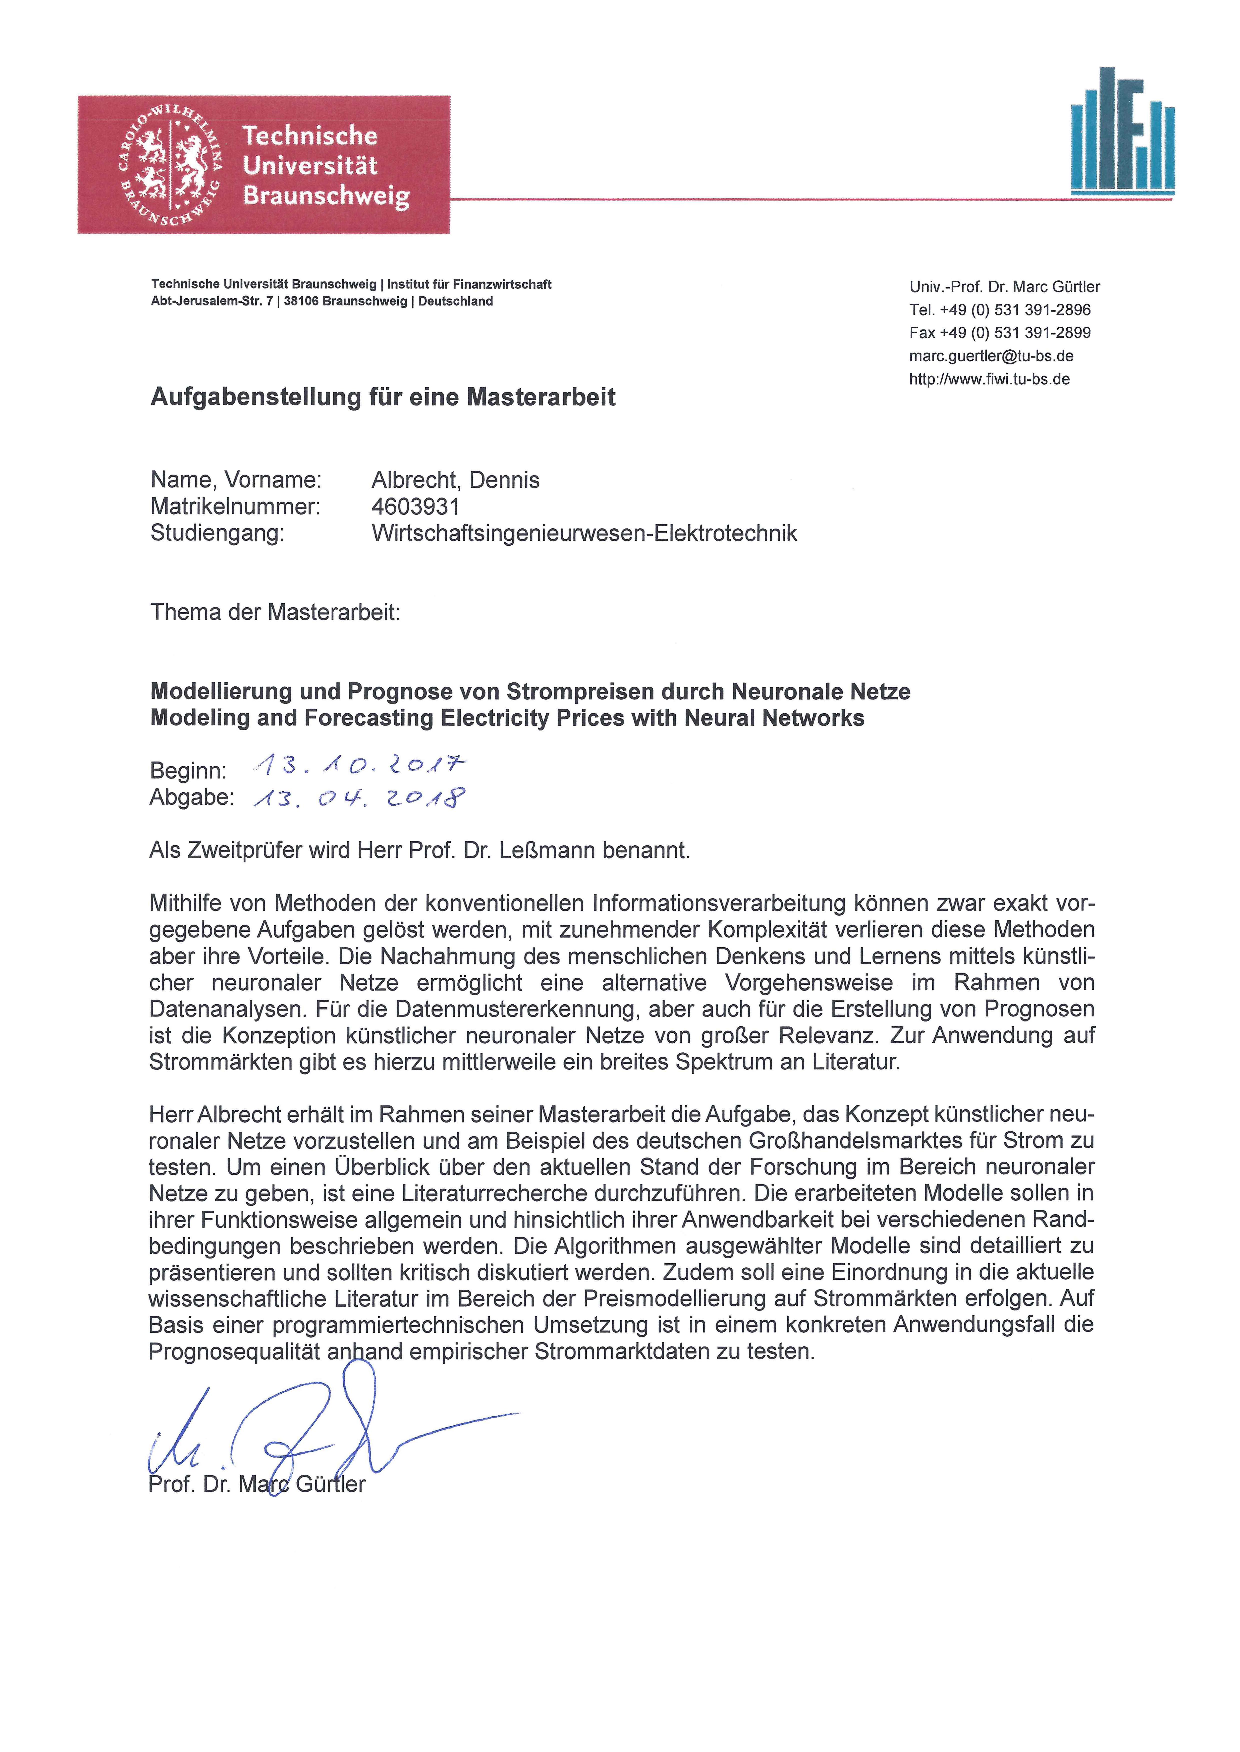
\includepdf[pages=-]{Bilder/Offiziell/Aufgabenstellung_Masterarbeit_600dpi_rot.pdf}    % Fügt alle Seiten des PDF Dokumentes ein

%---------------------------------------------------------------------------------
\newpage
%---------------------------------------------------------------------------------
%% Eidesstattliche Erklärung

%\thispagestyle{empty}
\pagenumbering{Roman}
\setcounter{page}{4}

{\LARGE \textbf{Eidesstattliche Erklärung}}\\ \vspace{1cm}

Ich erkläre hiermit an Eides statt, dass ich die vorliegende  Masterarbeit „\titel“ selbstständig verfasst sowie alle benutzten Quellen und Hilfsmittel vollständig angegeben habe.\\ \vspace{1cm}

Braunschweig, den \abgabedatum\\ \vspace{1cm}

\name
%---------------------------------------------------------------------------------  

%---------------------------------------------------------------------------------
\newpage
%---------------------------------------------------------------------------------
%% Vorlauf

\pagenumbering{Roman}

% !TEX root = 00_arbeit.tex

%---------------------------------------------------------------------------------
%% Inhaltsverzeichniss

\setcounter{page}{5}
{
\setstretch{1.3} 
\tableofcontents%
}
{
\setstretch{1.27} 
\newpage
\printglossary[type=abbreviations, title={Abkürzungsverzeichnis}]%
\newpage
\listoffigures%
\newpage
\listoftables%
\newpage
\printglossary[type=symbols,  nopostdot=false, title={Variablenverzeichnis}]%style=superborder,
}




%---------------------------------------------------------------------------------
\newpage
%---------------------------------------------------------------------------------
%% Hauptteil

\pagenumbering{arabic}

% !TEX root = 00_arbeit.tex

%---------------------------------------------------------------------------------
%% Einleitung

\section{Einleitung}

\blankpage
\blankpage

% Der Theorieteil wird informativ gehalten wobei ausgewählte Algorithmen im nachgang mathematisch vorgestellt werden.
% !TEX root = 00_arbeit.tex

%---------------------------------------------------------------------------------
%% Theorie

\section{Neuronale Netze}
%\farbig{[Erklärung der neuronalen Netze... vielfältige Anwendungsgebiete... Hier erforderlich Netze zur Zeitreihenvorhersage]}
%\setlength{\intextsep}{0pt}%
\begin{wrapfigure}{r}{0.5\textwidth}
    \centering
        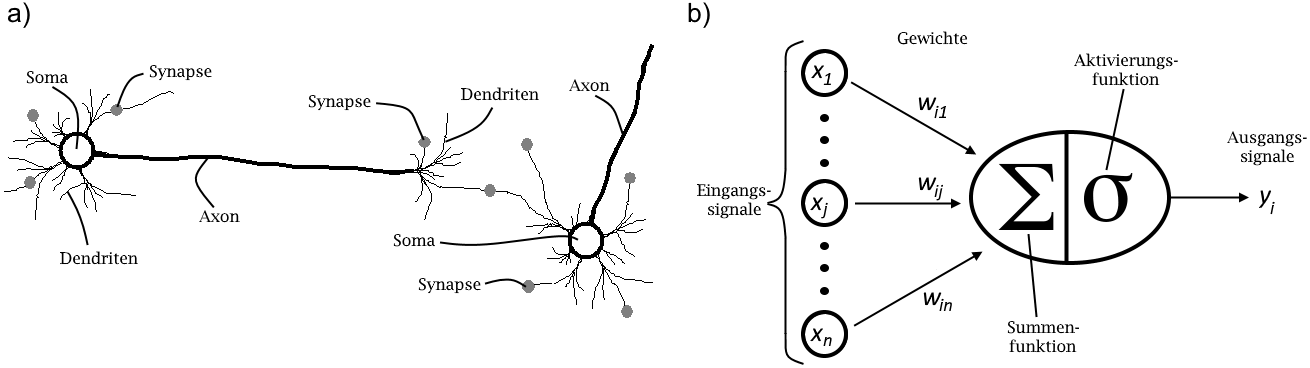
\includegraphics[width=0.5\textwidth]{Bilder/BNN_ANN.png}
    \caption{Gegenüberstellung eines Ausschnittes aus einem biologischen neuronalen Netz a)\protect\footnotemark{} und einem künstlichen neuronalen Netz b).}
    \label{fig:BNN_ANN}
\end{wrapfigure}

\addtocounter{footnote}{-1}%  -1 mal die Gesamtanzahl an Fußnoten in der wrapfigure
\addtocounter{Hfootnote}{-1}% -1 times total number of footnote(mark)s in the wrapfigure
\wrapfigfoot\footnotetext{\autoref{fig:BNN_ANN} a) und \autoref{tab:BNN_ANN} wurden aus\citet[2]{sen_an} übersetzt und angepasst.}
%\citet[\pno~2~ff.]{sen_an}

Ein künstliches neuronales Netz (engl. artificial neural networks)~(NN) ist ein mathematische Konstrukt. Es bildet ein informationsverarbeitendes System welches aus einer Vielzahl einfacher Einheiten den sogenannten Neuronen besteht. Entstanden ist es Anfang der 40er Jahre des letzten Jahrhunderts\fcite[A1.1:1]{Fiesler96} aus der Untersuchung von biologischen Abläufen im Nervensystem von Wirbeltieren, wo Sinneseindrücke des Körpers aufgenommen und mit Hilfe diverser neuronaler Netze verarbeitet werden. 
\autoref{fig:BNN_ANN} zeigt eine Gegenüberstellung eines künstlichen und biologischen Neurons und \autoref{tab:BNN_ANN} die Analogie seiner Bestandteile. Das zurzeit prominenteste künstliche Neuron (die kleinste Einheit im Netzwerk), dargestellt in \hbox{\autoref{fig:BNN_ANN} b)}, wird nach \citet{perceptron_ros58} als Perzeptron bezeichnet. Es summiert zunächst die gewichteten Eingänge mit $\varphi (x)=\sum_{i=1}^{n}x_{i}\omega_{i}$, anschließend wird die gewichtete Summe~$\varphi(x)$ über die Aktivierungsfunktion~$\sigma(x)$ als Ausgang~$y$ an das nächste Neuron übergeben.%

\setlength{\intextsep}{0pt}%
%\setlength{\columnsep}{10pt}%
\begin{wraptable}{l}{6.4cm}
    \caption {Analogie zwischen biologischen und künstlichen Neuronen.}
    \begin{tabular}{>{\centering\arraybackslash}m{2.2cm}>{\centering\arraybackslash}m{3.4cm}}
    \hline
    Biologisches\newline Neuron & Künstliches\newline Neuron            \\ \hline \hline
    Soma                & Summen- und\newline Aktivierungsfunktion      \\ 
    Dendrit             & Eingang                                       \\ 
    Axon                & Ausgang                                       \\ 
    Synapse             & Gewicht                                       \\ \hline
    \end{tabular}
    \label{tab:BNN_ANN}
\end{wraptable}

Klassische Aktivierungsfunktionen sind dabei die \hbox{Heaviside-,} die lineare Schwellwert-, die Fermifunktion und der Tangens Hyperbolicus\footnote{Vgl. \citet[5]{neuralnet_intro} und \citet[39 f]{dkriesel07}.}.\\

Es gibt Problemstellungen die mit klassischen mathematischen Modellen und Algorithmen gar nicht oder nur schwer zu lösen sind. Neuronale Netze unterscheiden sich zu klassischen Algorithmen durch ihre Lernfähigkeit. Ohne explizite Programmierung sind sie in der Lage eine Aufgabe anhand von Trainingsbeispielen zu erlernen. Einige Beispiele wären die Gesichtserkennung oder die Erkennung von menschlicher Sprache.
\newpage

Künstliche neuronale Netze sind augenblicklich eine Disziplin der Computional Intelligence~(CI), welches wiederum einen Teilbereich der Künstlichenintelligenz (artificial intelligence)~(AI) darstellt. Diese fasst verschiedene von der Natur inspirierte Berechnungsmethoden zusammen. Weitere Methoden der CI sind Fuzzy-Systeme~(FS), Evolutionäre Algorithmen~(EA), Schwarmintelligenz~(SI) und Künstliche Immunsysteme~(AIS).\fcite[11 ff]{Kroll16} Obwohl sich diese Arbeit wesentlich mit NN beschäftigen wird, wird an dieser Stelle auf weitere CI-Methoden hingewiesen, da in der Literatur hybride CI-Systeme bekannt sind und auch genutzt werden.

\subsection{Charakterisierung und Anwendung künstlicher neuronaler Netze}

Da es nicht das NN gibt sondern viele unterschiedliche Arten, die teilweise spezielle Anwendungsgebiete finden, werden in diesem Unterkapitel Charakterisierungskriterien für NN vorgestellt. Schließlich wird ein Überblick über mögliche Anwendungsgebiete gegeben.\\

Im allgemeinen können NN anhand der folgenden drei Kriterien charakterisiert werden\fcite[7 ff]{characterisation_4}:%

\begin{enumerate}
\item%
Nach der Art des verwendeten Neurons.\\
Dazu gibt es in der Literatur vielfältige Beispiele. \citet{Fiesler96} zählen einige Beispiele im Kapitel B1 auf und weisen auf Unterschiede hin. Als Beispiel wird dort das bereits erwähnte Perceptron beschrieben. Dann gehen sie auf das Neuron des Hopfield-Netzwerkes ein, bei dem das Neuron ein Teilchen beschreibt welches sich in einem Magnetfeld ausrichtet. Ein eher exotischer Vertreter der dort nicht erwähnt wird ist das Fuzzy-Neuron von \citet{fuzzy-neuron}, welches nach der Aktivierung mehrere mögliche Zustände einnehmen kann und seine Anwendung in der Mustererkennug findet.

\item%
Nach der Topologie buw. der Verbindungsarchitektur.\\
Sie beschreibt wie Neuronen in einem Netzwerk verbunden sind.
Es werden folgende Architekturen unterschieden:
\begin{itemize}
\item[\textbf{$\bullet$}]%
Autoassoziative: Hierbei fungieren die Eingangs- gleichzeitig als Ausgangsneurone (z.B. das Hopfield-Netzwerk). 

\item[\textbf{$\bullet$}]%
Heteroassoziative: Unterschiedliche Neurone übernehmen die Rolle der Eingangs- bzw. Ausgangsneurone. Hierzu zählen die Multylayer-Perzeptrons (MLP) bei dem mehrere Schichten von mehrzahligen Perzeptronen ein Netzwerk Bilden\fcite[86 ff]{dkriesel07}. Aber auch das Kohonen Netzwerk auch bekannt als Self Organizing Maps (SOM) bei dem die Neuronen sich selbständig anordnen und der Zustand des Netzes als Ausgabe dient\fcite[153 ff]{dkriesel07}.

Zusätzlich wird unterschieden wie die Verbindungen unter den einzelnen Neuronen realisiert sind. Hier wird zwischen zwei Arten unterschieden:

\item[$\circ$]%
Feedforward: Diese Netzwerke bestehen meistens aus Schichten und eine Schicht ist nur mit der jeweils nächsten Schicht verbunden.

\item[$\circ$]%
Recurrent (Feedback): In der deutschsprachigen Literatur als rückgekoppelte oder rekurrente Netze bezeichnet beeinflussen sich diese Netzwerke selbst. Die Neuronen dieser Netzwerke besitzen eine Verbindung entweder zu sich selbst (direkte Rückkoppelung), zu den Neuronen der vorhergehenden Schicht (indirekte Rückkopplung), zu den Neuronen der gleichen Schicht (laterale Rückkopplung) oder vollständig verbundene Netze (Verbindungen zwischen allen Neuronen ausgenommen der direkten Rückkopplung). Durch die Rückkopplung besitzen diese Netzwerke ein "Gedächtnis"~da der vorherige Zustand in die Auswertung der aktuellen Eingangsinformation mit einfließt.\fcite[42 ff]{dkriesel07} Ein Beispiel für ein vollständig verbundenes Netzwerk ist das Hopfield-Netzwerk.

\end{itemize}

\item%
Nach dem Lernalgorithmus. Dieser ermöglicht es das Netzwerk zu trainieren. Die heutzutage benutzten Algorithmen werden in drei Gruppen unterteilt\footnote{Vgl. \citet[55]{dkriesel07}.\label{kriesel55}}:

\begin{itemize}
\item[\textbf{$\bullet$}]%
Supervised learning (überwachtes Lernen): Die Trainingsbeispiele bestehen aus einer Menge an Eingangsinformationen und den dazugehörigen Ausbangsinformationen. Das Ziel ist es die Differenz zwischen der tatsächlichen Ausgabe des Netzwerks und den vorliegenden Ausgangsinformationen zu minimieren.

\item[\textbf{$\bullet$}]%
Reinforcement learning (bestärkendes Lernen): Plakativ kann diese Lernmethode als Zuckerbrot und Peitsche bezeichnet werden bzw. lernen durch Belohnung und Bestrafung. Hierbei werden die Eingangsinformationen zur Verfügung gestellt und die Ausgabe des Netzwerkes wird anhand einer Belohnungsfunktion bewertet. Wird die Ausgabe als gut/schlecht angesehen so werden die zugehörigen Verbindungen gestärkt/geschwächt\footnote{Vgl. \citet[201]{dkriesel07} und \citet[A2.3:5]{Fiesler96}.}. 

\item[\textbf{$\bullet$}]%
Unsupervised learning (unüberwachtes Lernen): Wird auch als selbstorganisiertes (self organized) Lernen bezeichnet. Die Trainingsbeispiele bestehen hierbei nur aus Eingansinformationen. Das Netzwerk versucht aus den Eingansinformationen selbstständig Ähnlichkeiten zu erkennen.
Unüberwachte Lernmethoden werden noch unterteilt in konkurrierendes (competitive) und nicht konkurrierendes (noncompetitive) Lernverfahren. Der unterschied besteht darin dass bei dem konkurrierenden Verfahren in einem Netzwerk einzelne Gruppen von Neuronen um die Aktivität konkurrieren\fcite[B3.3:5]{Fiesler96}.

Zusätzlich unterscheidet man unter allen drei Lernmethoden zwei Lernarten\fcite[A2.3:3]{Fiesler96}: 
\item[$\circ$]%
off-line learning: Auch Batch-Trainingsverfahren genannt. Hierbei wird die Netzwerkausgabe nach einer Menge von Eingangsinformationnen ausgewertet und anschließend werden die Gewichte angepasst.

\item[$\circ$]%
on-line learning: Hier werden die Gewichte nach jeder einzelnen Beobachtung der gesamten Eingangsinformationen angepasst. 

\end{itemize}

\end{enumerate}

Vollständigkeitshalber wird erwähnt dass \citet{characterisation_4} vier Charakterisierungskriterien nennen. Wobei als viertes Kriterium der Informationsgewinnungsalgorithmus (recall algorithm) aufgeführt ist. In dieser Arbeit wird auf dieses Kriterium verzichtet, da weder \citet{characterisation_4} Einteilung/Auflistung aufführen noch in anderer Literatur dieses Kriterium eine Erwähnung findet.\\

Es gibt vielfältige Anwendungsgebiete für NN. Angefangen bei Optimierungsproblemen, wo das Ziel es ist optimale Werte für ein gegebenes System zu finden. Über die Datenverarbeiteung, wo Bild- bzw. Sprachinformationen verarbeitet, generiert oder komprimiert werden sollen. Bis zur Klassifikation/Erkennung von Mustern, wo es darum geht aus einer Dantemenge zusammenhängende Muster zu erkennen. Weitere Anwendungen sind die Kontrelle/Regelung von industriellen Anlagen und die wichtigste (bezogen auf diese Arbeit) ist die Funktionsapproximation bzw. Zeitreihenmodellierung, wo die Beziehung aus Eingangsinformationen und dem gewünschtem Ausgang zu finden gilt. Dies sind einige kurz umrissene Anwendungsbeispiele. In der Literatur werden deutlich mehr aufgeführt.\footnote{Vgl. \citet[224]{Kroll16}, \citet[15]{comp_int_07} und \citet[F1 ff]{Fiesler96}.}\\

%\farbig{NN sind Black-Box und Analyse ist schwer aber es gibt in der Literatur mögliche Analyseverfahren.}


\subsection{Gängige Modelle}

\subsubsection{Multilayerperzeptrons (MLP)}

\subsubsection{Radiale Basisfunktionen (RBF)}

\subsubsection{Self Organizing Maps (SOM)}

\subsubsection{Hopfield-Netzwerk}


%\lipsum


%\subsection{Multilayerperzeptrons (MLP)}

%\subsection{Radiale Basisfunktionen (RBF)}

%\subsection{Gegenüberstellung von MLP- und RBF-Netzen}

%% !TEX root = 00_arbeit.tex

%---------------------------------------------------------------------------------
%% Strommarkt

\section{Algorithmen ausgewählter Modelle} 
%% !TEX root = 00_arbeit.tex

%---------------------------------------------------------------------------------
%% Stata

\section{Aktuelle Preismodellierung auf Strommärkten}
%% !TEX root = 00_arbeit.tex

%---------------------------------------------------------------------------------
%% Diskussion

\section{Umsetzung in Stata} 
%%% !TEX root = 00_arbeit.tex

%---------------------------------------------------------------------------------
%% Diskussion

\section{Diskussion} 
%% !TEX root = 00_arbeit.tex

%---------------------------------------------------------------------------------
%% Zusammenfassung

\section{Zusammenfassung} 

Da aber die Differenzen der Schätzer im niedrigen einstelligen Bereich liegen, weisen sie eine geringe Abweichung auf. Aus diesem Grund lassen die Ergebnisse hieraus keine Bewertung darüber treffen ob eines der beiden vorgestellten Lernalgorithmen generell zu besseren Ergebnissen führt. Dieses Ergebnis war zu erwarten da das zugrundeliegende Netzwerk gleich bleibt und sie Art und Weise wie die Gewichte verändert wurden variiert wurde. 
%% !TEX root = 00_arbeit.tex

%---------------------------------------------------------------------------------
%% Ausblick

\section{Ausblick} 

%---------------------------------------------------------------------------------
\newpage
%---------------------------------------------------------------------------------
%% Schluss

\pagenumbering{roman}

\section{Literaturverzeichnis}

\printbibliography


%\bibliographystyle{alpha}               % Stil des Literaturverzeichnisses 
%\bibliography{10_literatur}             % Aufruf des Literaturverzeichnisses

%---------------------------------------------------------------------------------
\newpage
%---------------------------------------------------------------------------------
%% Anhang

% !TEX root = 00_arbeit.tex

%---------------------------------------------------------------------------------
%% Inhaltsverzeichniss

\section{Anhang} 




%-------------
%% Einstellungen für die richtige Darstellung von Fußnoten und Hyperlinks
\AtEndDocument{%
\ifnum\value{Hfootnote}=\value{footnote}%OK
  \PackageInfo{footnote}{%
    Number of Hyperfootnotes \arabic{Hfootnote} = number of footnotes \arabic{footnote}!
    \MessageBreak%
    }
\else
  \PackageError{footnote}{%
    Hyperfootnote \arabic{Hfootnote} != footnote \arabic{footnote}!%
   }{Did you make a mistake with\MessageBreak%
     \string\footnotemark , \string\footnotetext , or \MessageBreak%
     \string\addtocounter { Hfootnote or footnote } ?%
   }
\fi%
%\thispagestyle{empty}    
}
%-------------
\end{document}
